\documentclass{beamer}
\usepackage{tcolorbox}
\usepackage{caption}
\usepackage{tikz}
\usepackage{pgfplots}
\usepackage{adjustbox}
\usepackage{pgfplots}
\usepackage{multicol}
%\beamerdefaultoverlayspecification{<+->}
\newcommand{\data}{\mathcal{D}}

\setlength{\abovedisplayskip}{1pt}
\setlength{\belowdisplayskip}{1pt}

\makeatletter
\def\magicomadjust{0em}  % a way to adjust if the spacing should be different
\newdimen\indent@amount
\def\magicom{\relax
  \ifhmode $$%
    \predisplaypenalty\@M \postdisplaypenalty\@M
    \abovedisplayskip-\baselineskip \belowdisplayskip\z@
    \abovedisplayshortskip\abovedisplayskip
    \belowdisplayshortskip\belowdisplayskip
    \global\indent@amount\predisplaysize
     $$\count@\prevgraf \advance\count@-\thr@@
         \prevgraf\count@
    \global\advance\indent@amount-2em  % correction for \predisplaysize indent
    \global\advance\indent@amount\magicomadjust  % correction for verse env, for example
    \hspace*\indent@amount
  \else\typeout{*Not in hmode*}\fi}
\makeatother



\DeclareMathOperator*{\argmin}{arg\,min}

\newcommand\Item[1][]{%
	\ifx\relax#1\relax  \item \else \item[#1] \fi
	\abovedisplayskip=0pt\abovedisplayshortskip=0pt~\vspace*{-\baselineskip}}


\usetheme{metropolis}           % Use metropolis theme


\title{Support Vector Machines}
\date{\today}
\author{Nipun Batra}
\institute{IIT Gandhinagar}

\begin{document}
\maketitle


\begin{frame}{Support Vector Machines}
\begin{itemize}
	\item Popular binary classification technique
\end{itemize}

\begin{figure}
\centering
\begin{overprint}
    \onslide<1>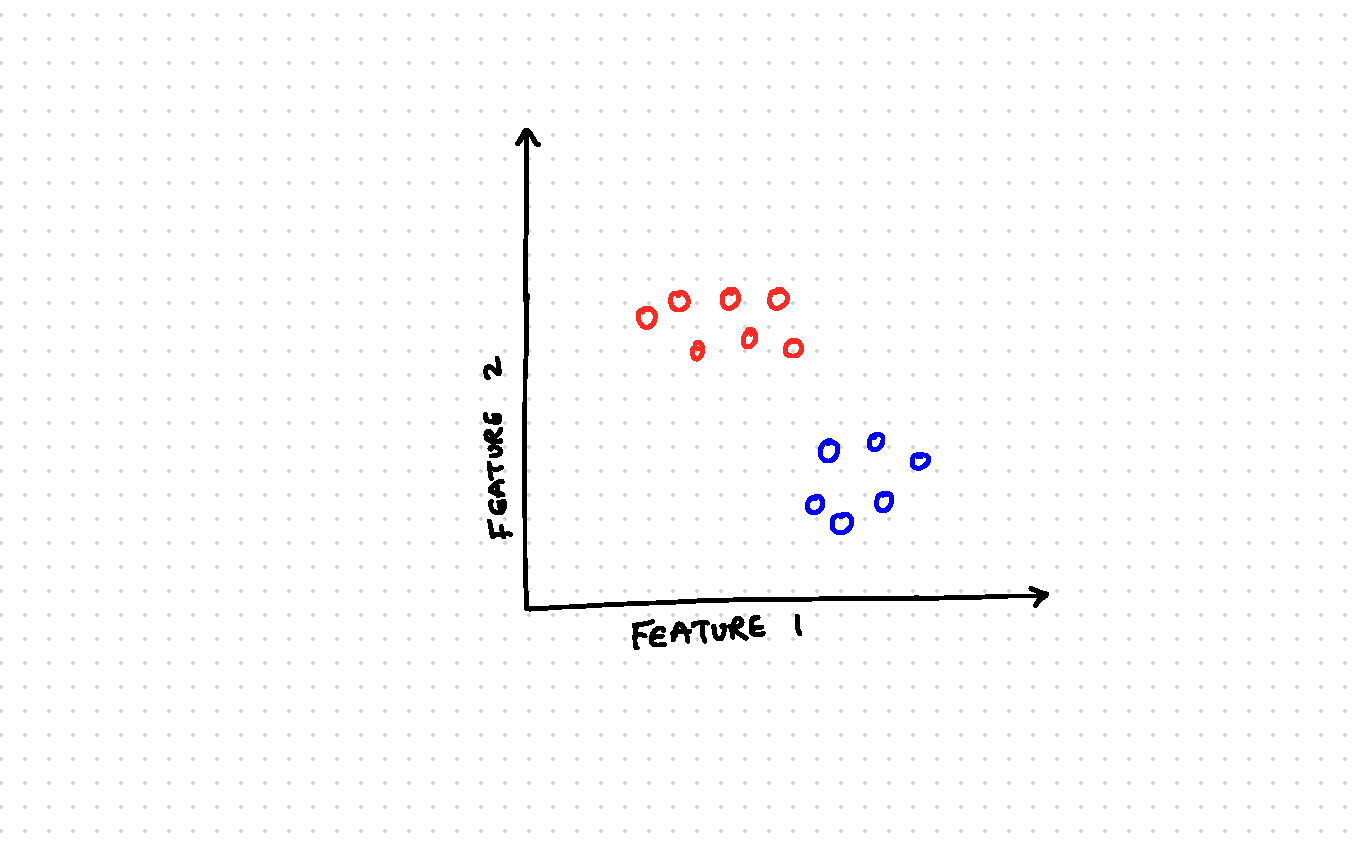
\includegraphics[scale = 0.3]{SVM/Svm-1.pdf}
    \onslide<2>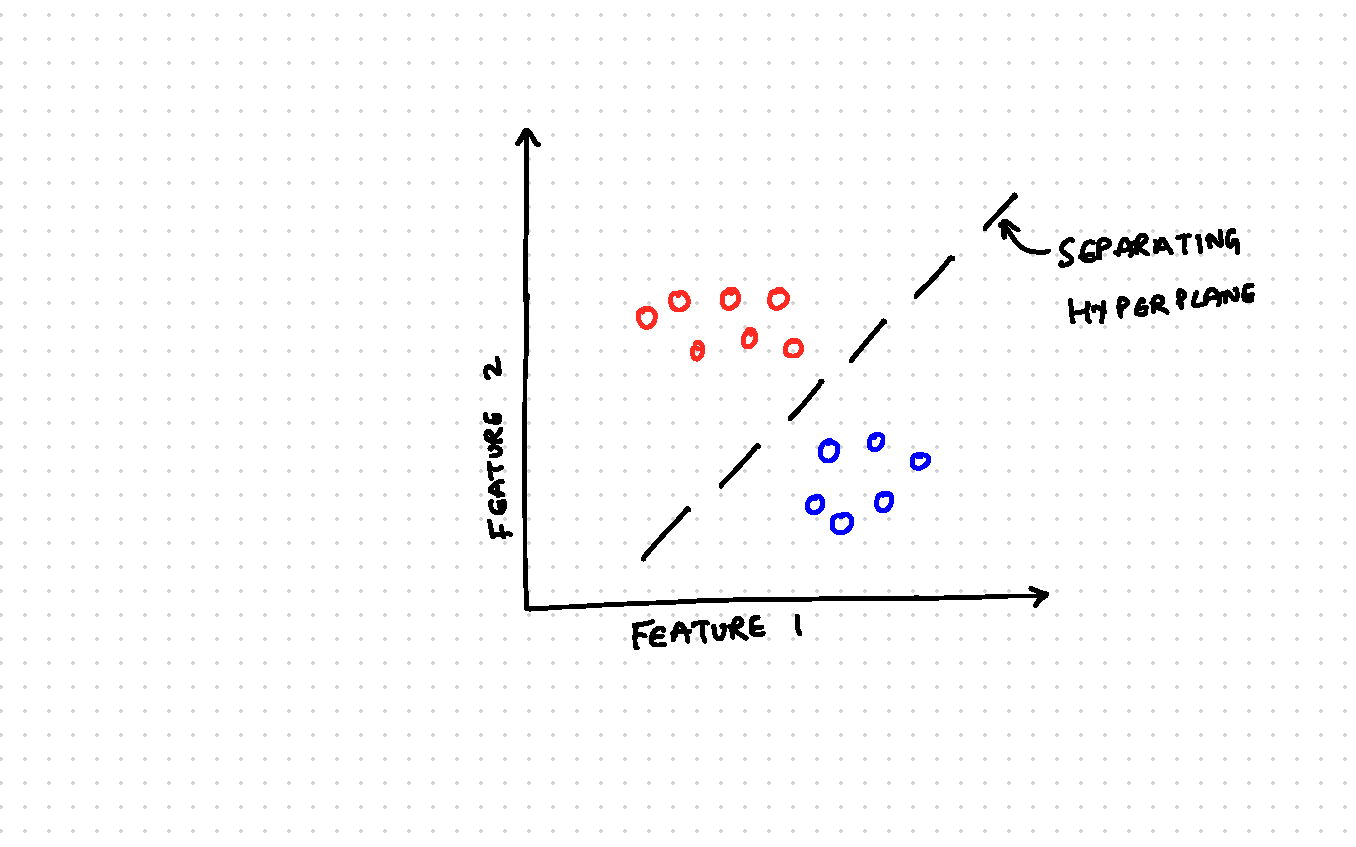
\includegraphics[scale = 0.3]{SVM/Svm-2.pdf}
    \onslide<3>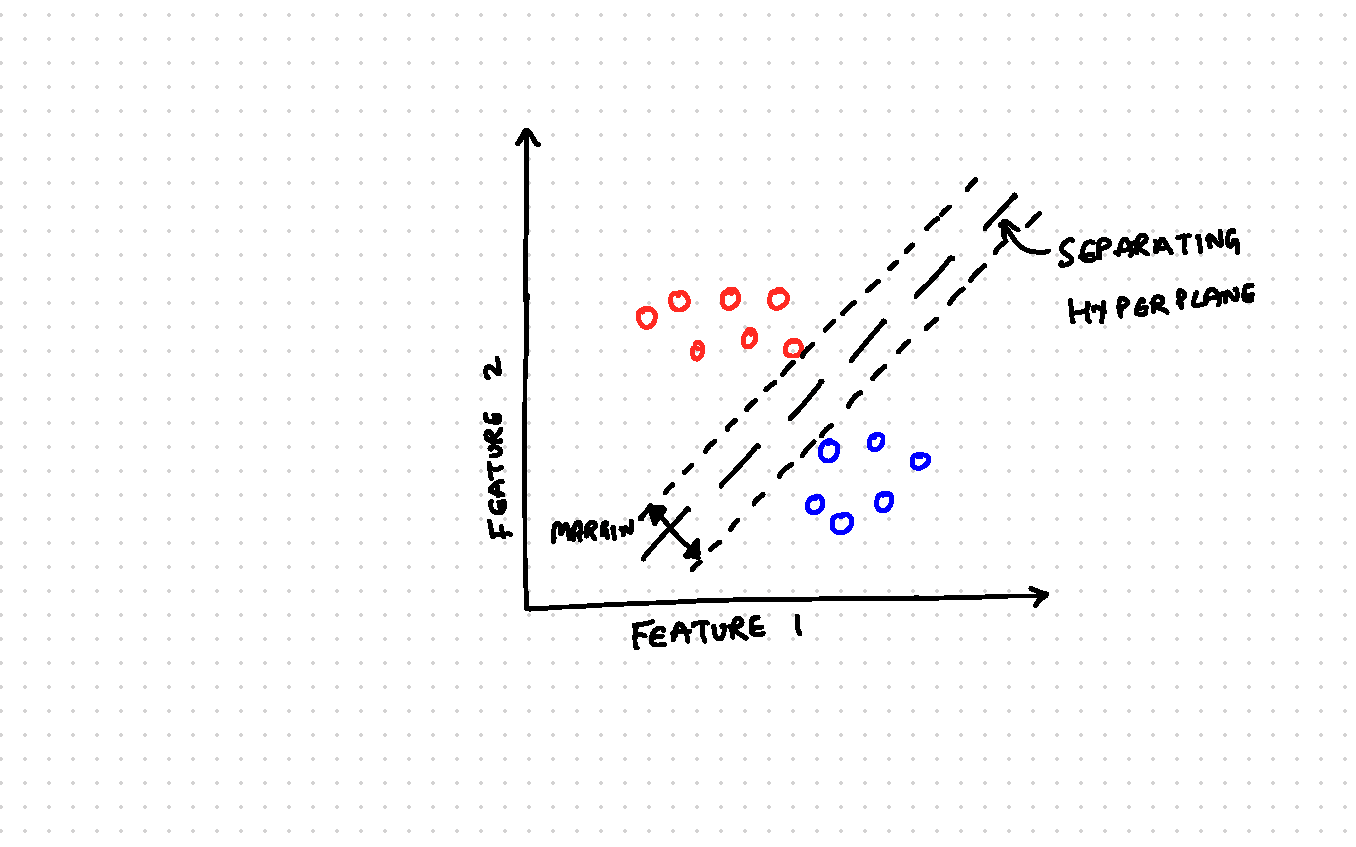
\includegraphics[scale = 0.3]{SVM/Svm-3.pdf}
    \onslide<4>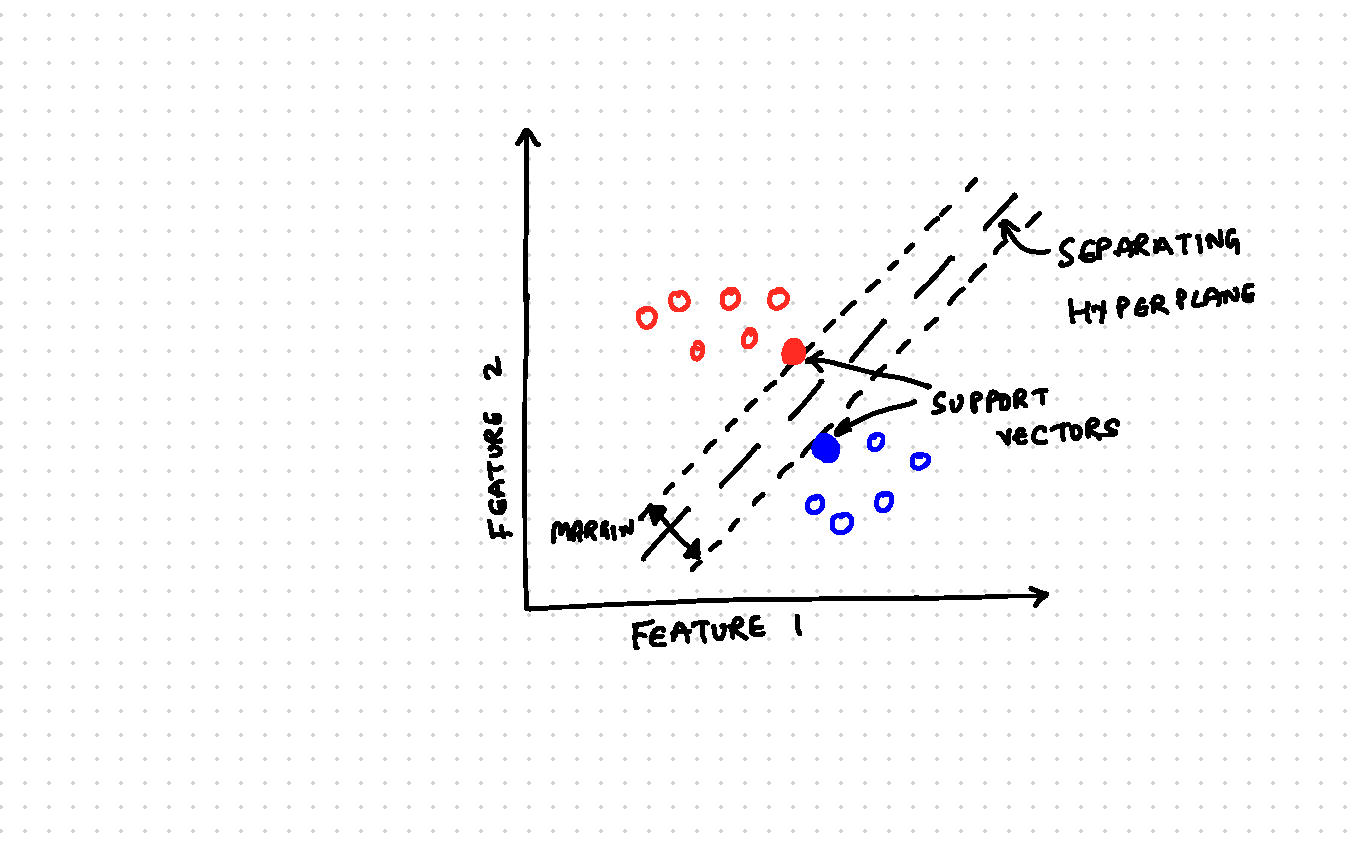
\includegraphics[scale = 0.3]{SVM/Svm-4.pdf}
    
    \end{overprint}
\end{figure}


\only<2->
{
  $\Rightarrow$Draw a separating hyperplane\\
 
}
\only<3->
{
  $\Rightarrow$Maximize the Margin
}

\end{frame}

\begin{frame}{Hyperplane v/s Dimensions}
\begin{figure}
    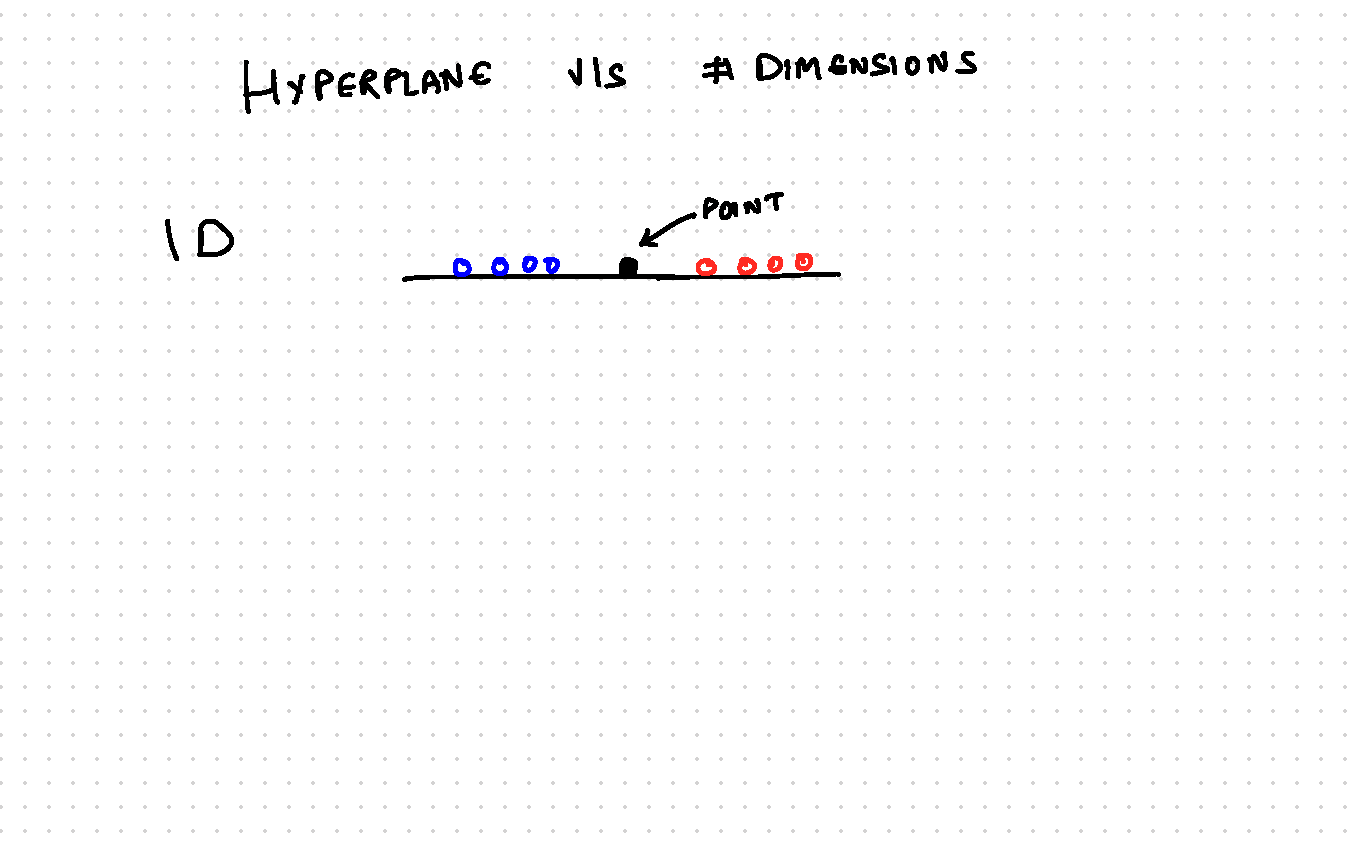
\includegraphics[width=\linewidth]{./SVM/Svm-5.pdf}  
\end{figure}
\end{frame}

\begin{frame}{Hyperplane v/s Dimensions}
\begin{figure}
    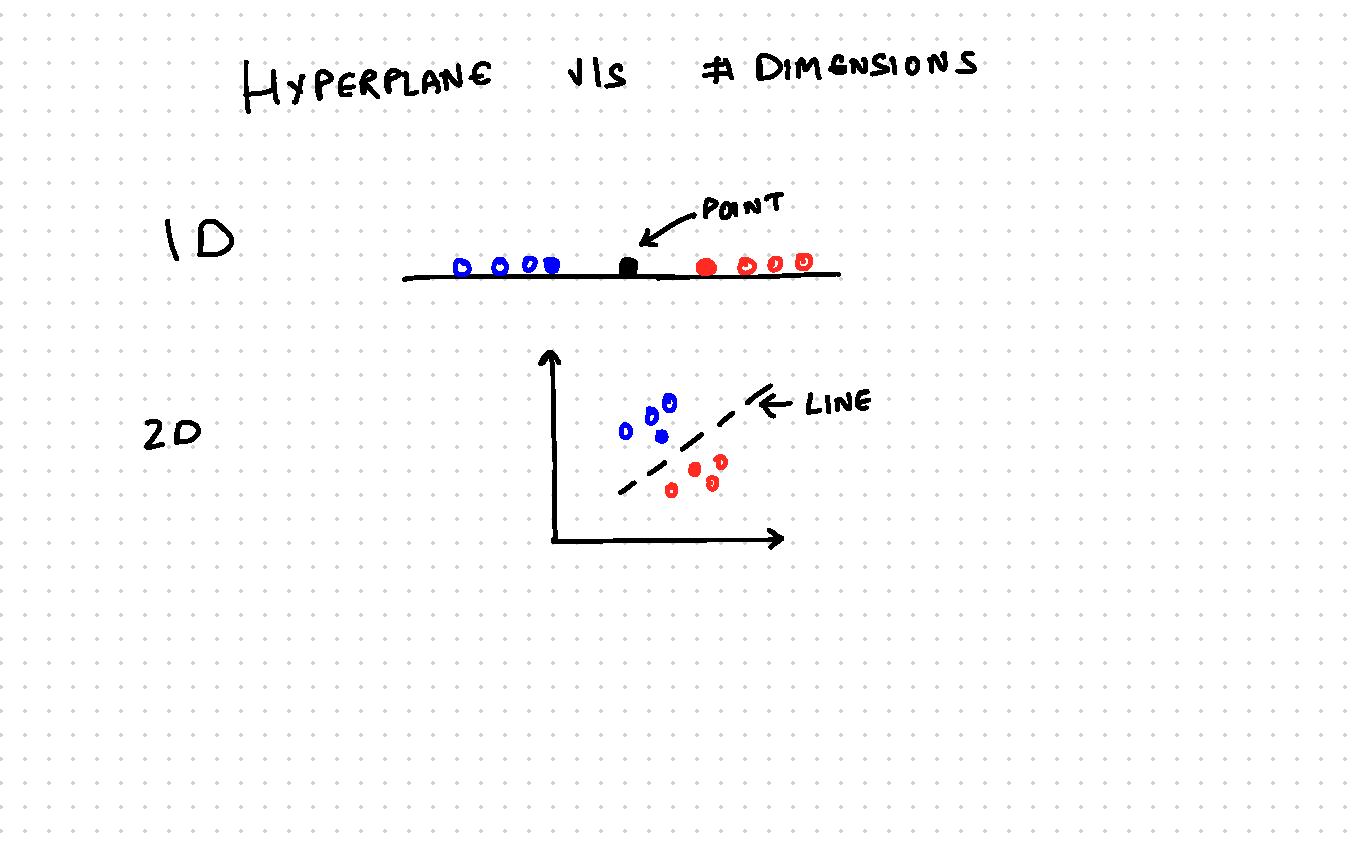
\includegraphics[width=\linewidth]{./SVM/Svm-6.pdf}  
\end{figure}
\end{frame}

\begin{frame}{Hyperplane v/s Dimensions}
\begin{figure}
    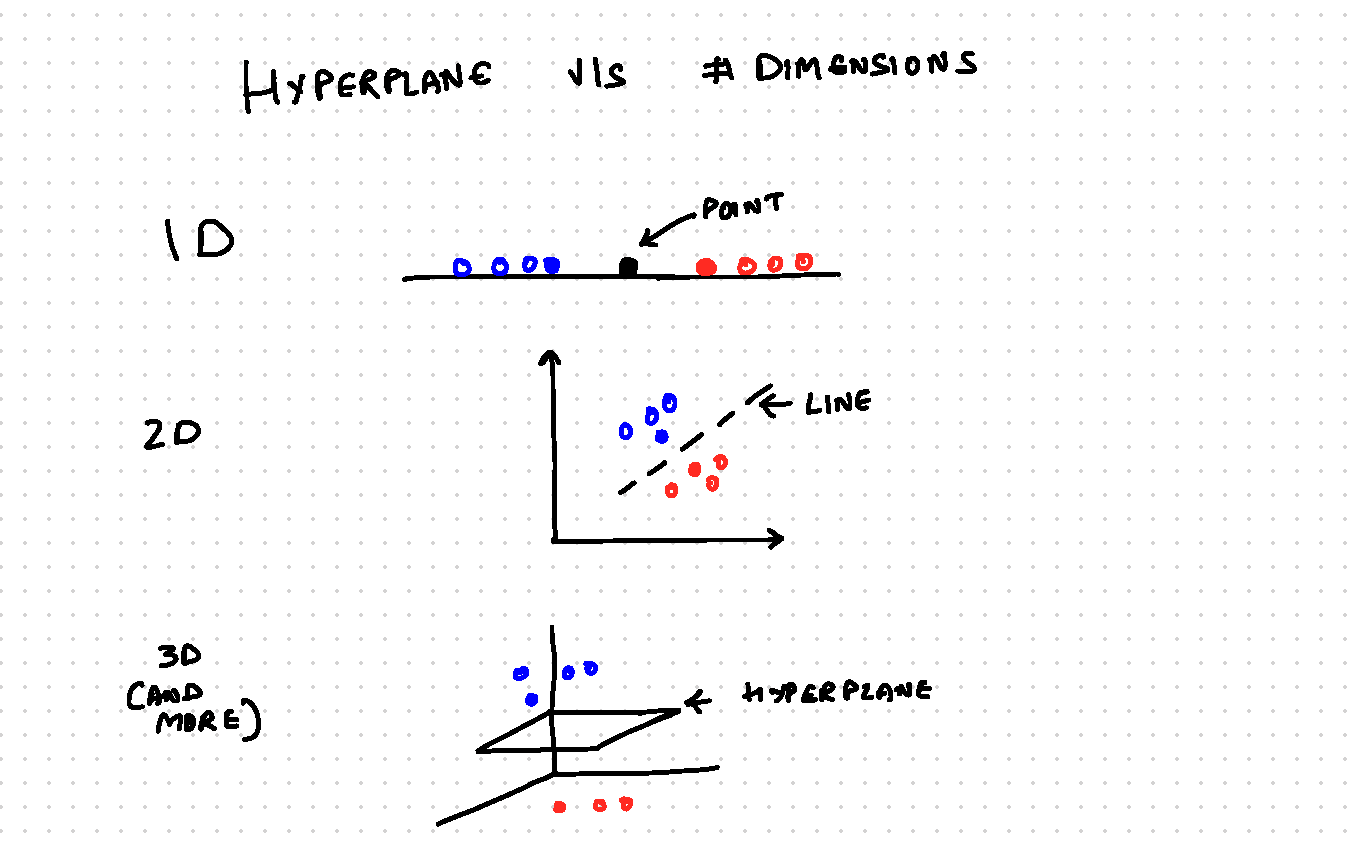
\includegraphics[width=\linewidth]{./SVM/Svm-7.pdf}  
\end{figure}
\end{frame}


\begin{frame}{Equation of a Hyperplane}

\begin{itemize}
	\item Defined by the point $P_{0}$ and the $\perp$ to the plane at that point $\overrightarrow{\text{w}}$
\end{itemize}

\begin{figure}
\begin{overprint}
\onslide<1> 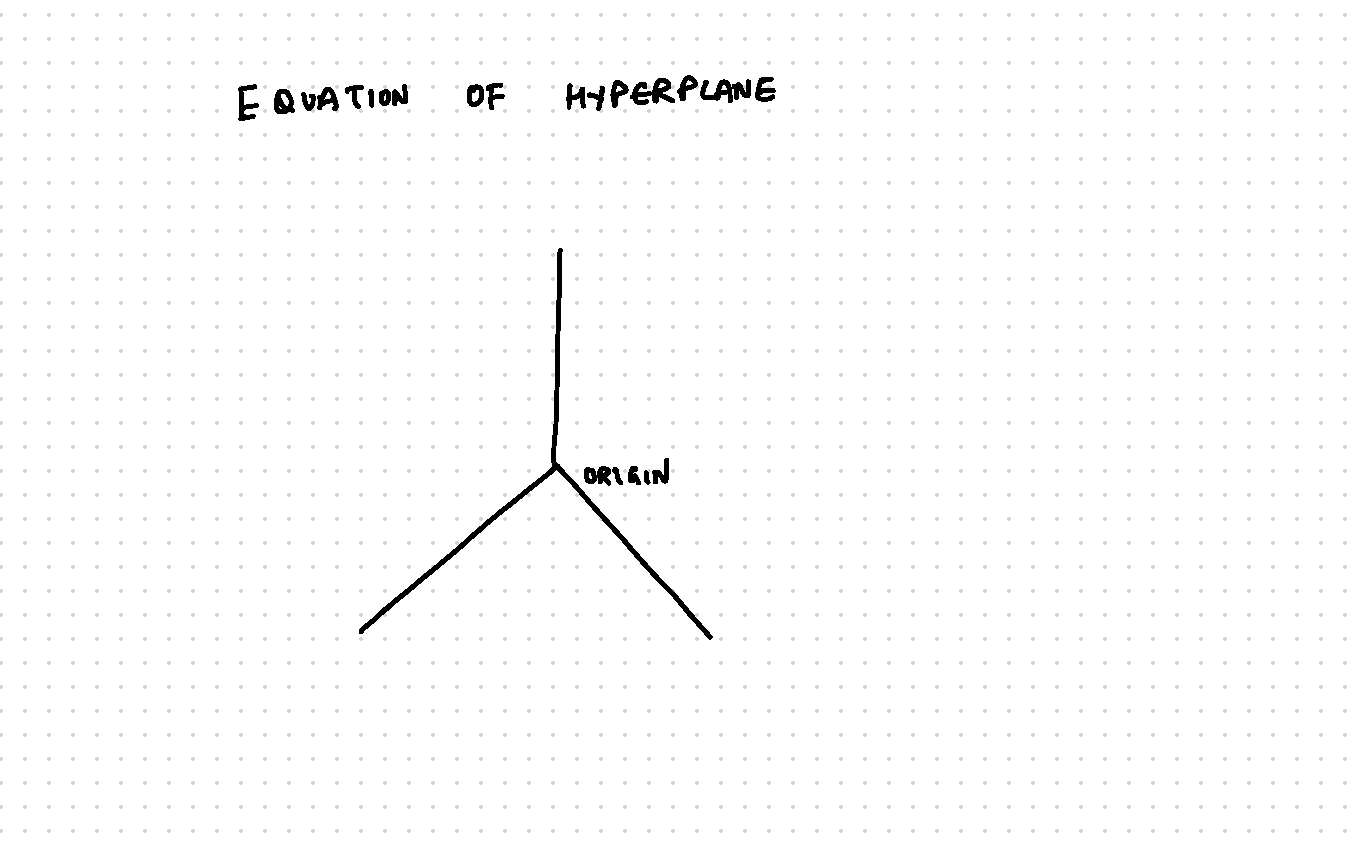
\includegraphics[scale=0.3]{./SVM/Svm-12.pdf}
\onslide<2> 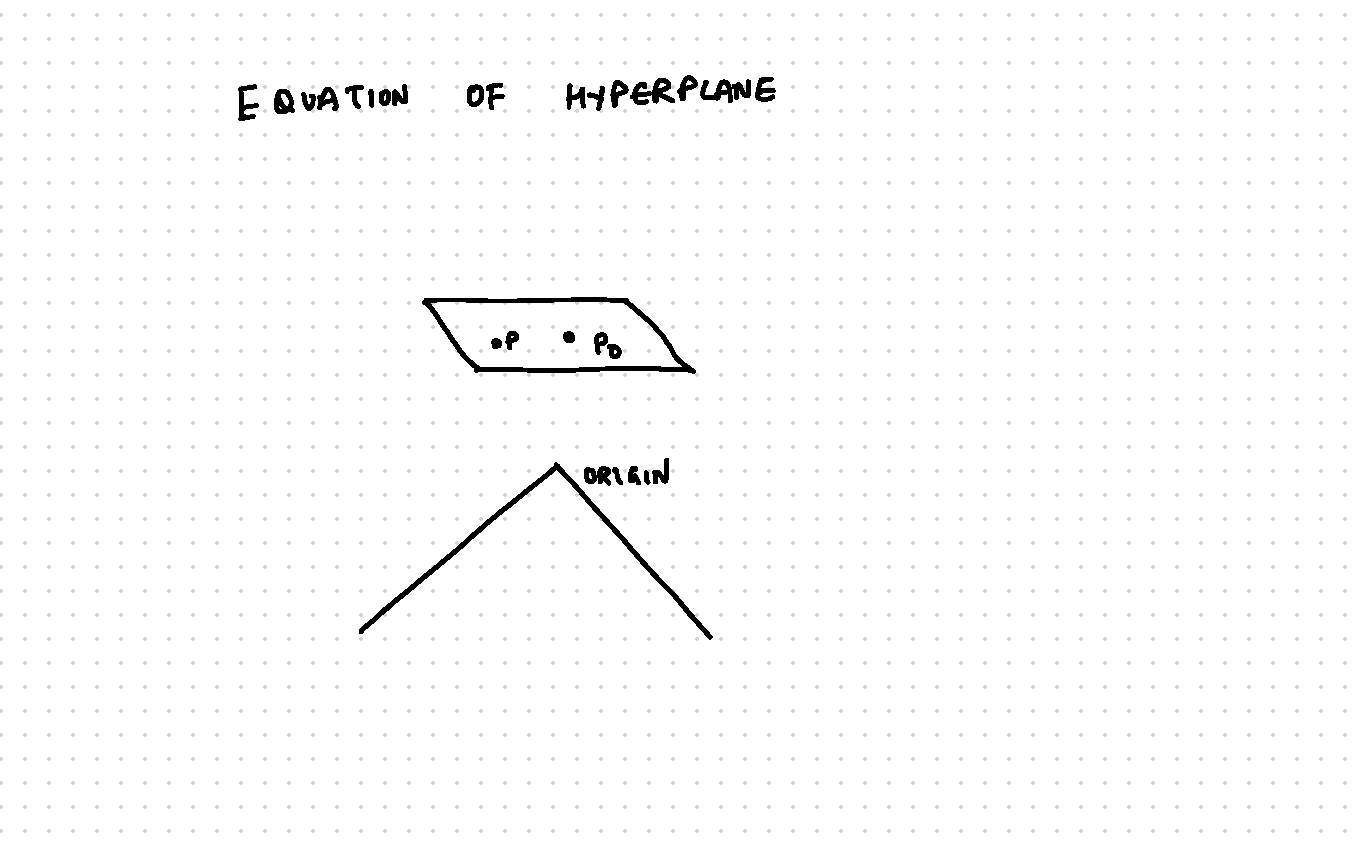
\includegraphics[scale=0.3]{./SVM/Svm-13.pdf}
\onslide<3> 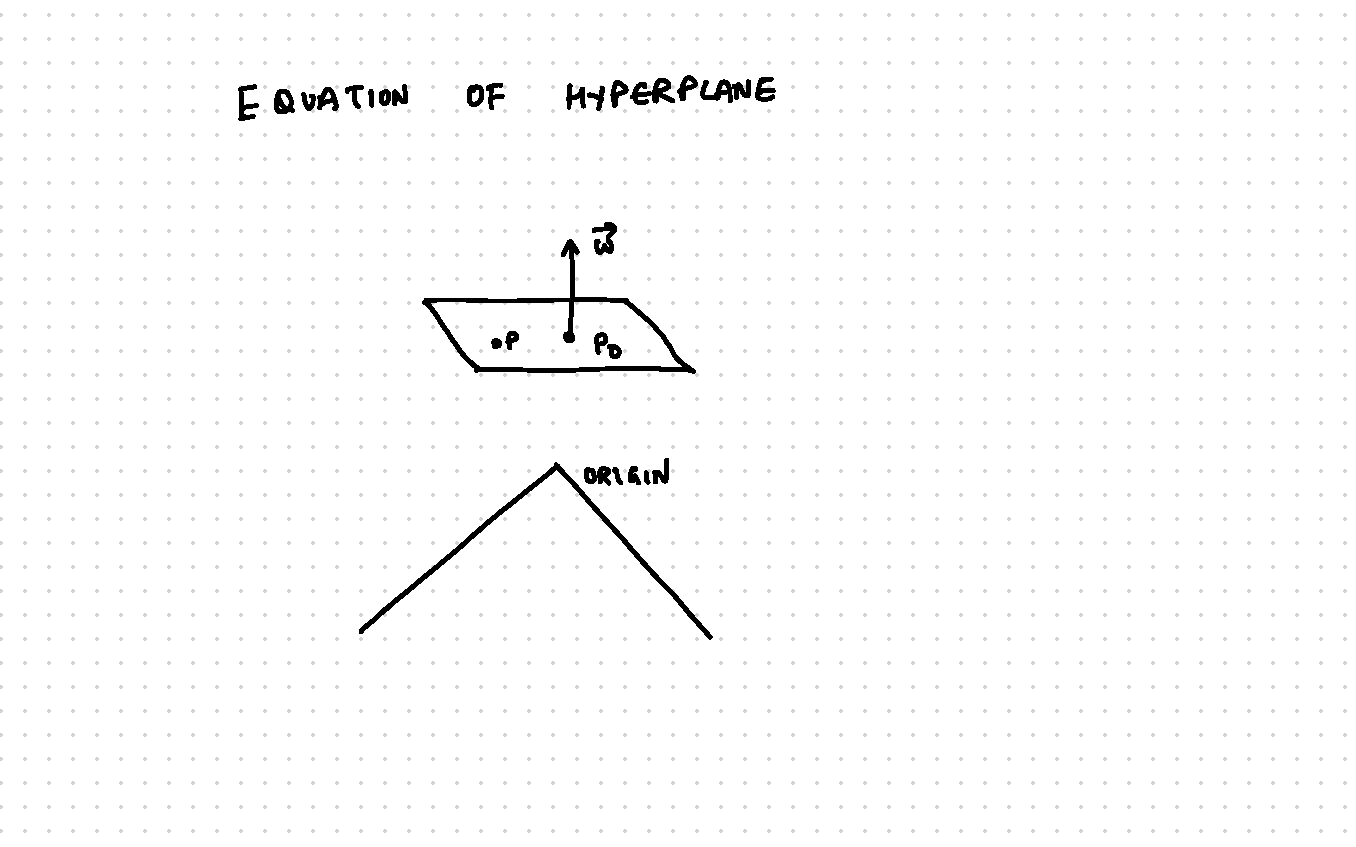
\includegraphics[scale=0.3]{./SVM/Svm-14.pdf}
\onslide<4> 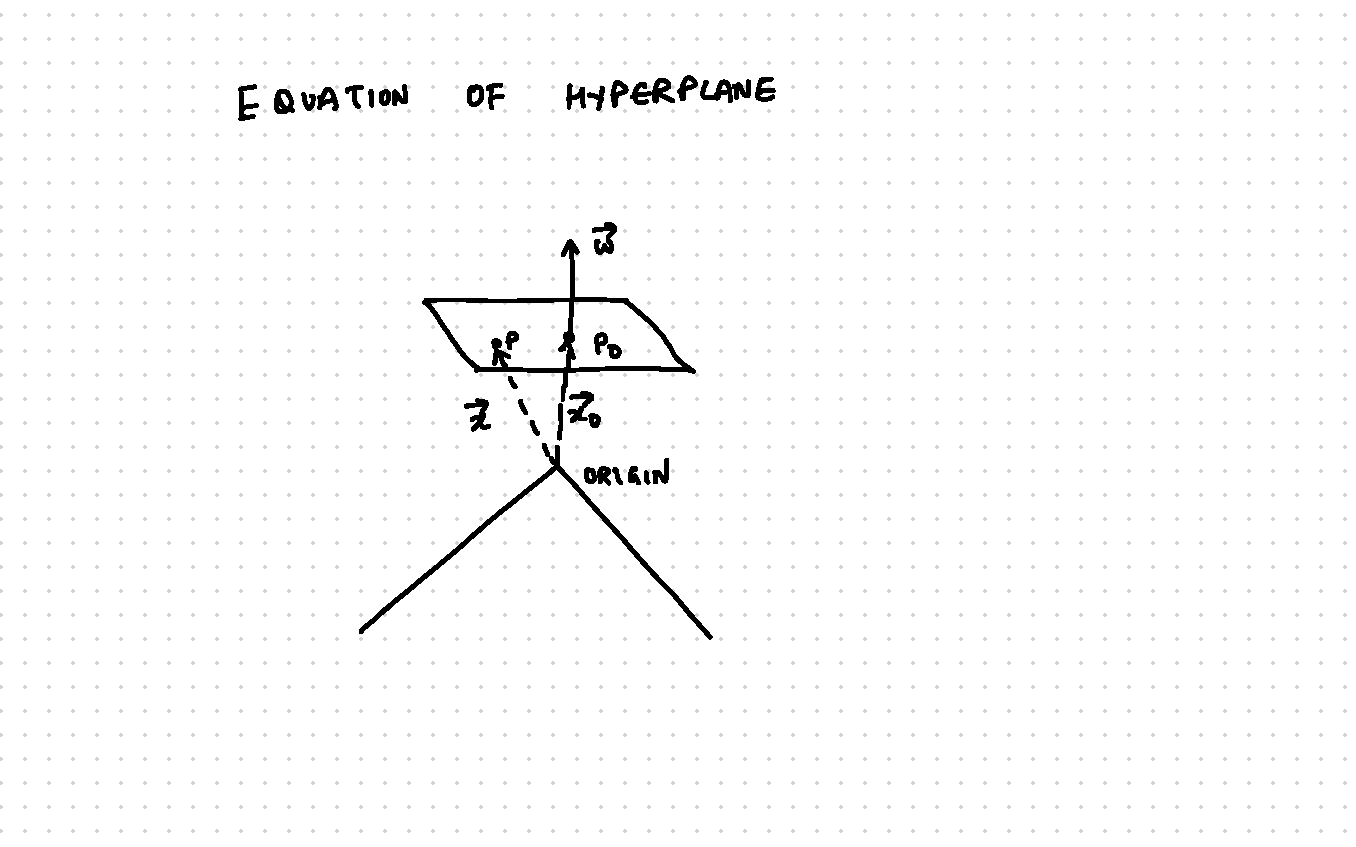
\includegraphics[scale=0.3]{./SVM/Svm-15.pdf}
\onslide<5> 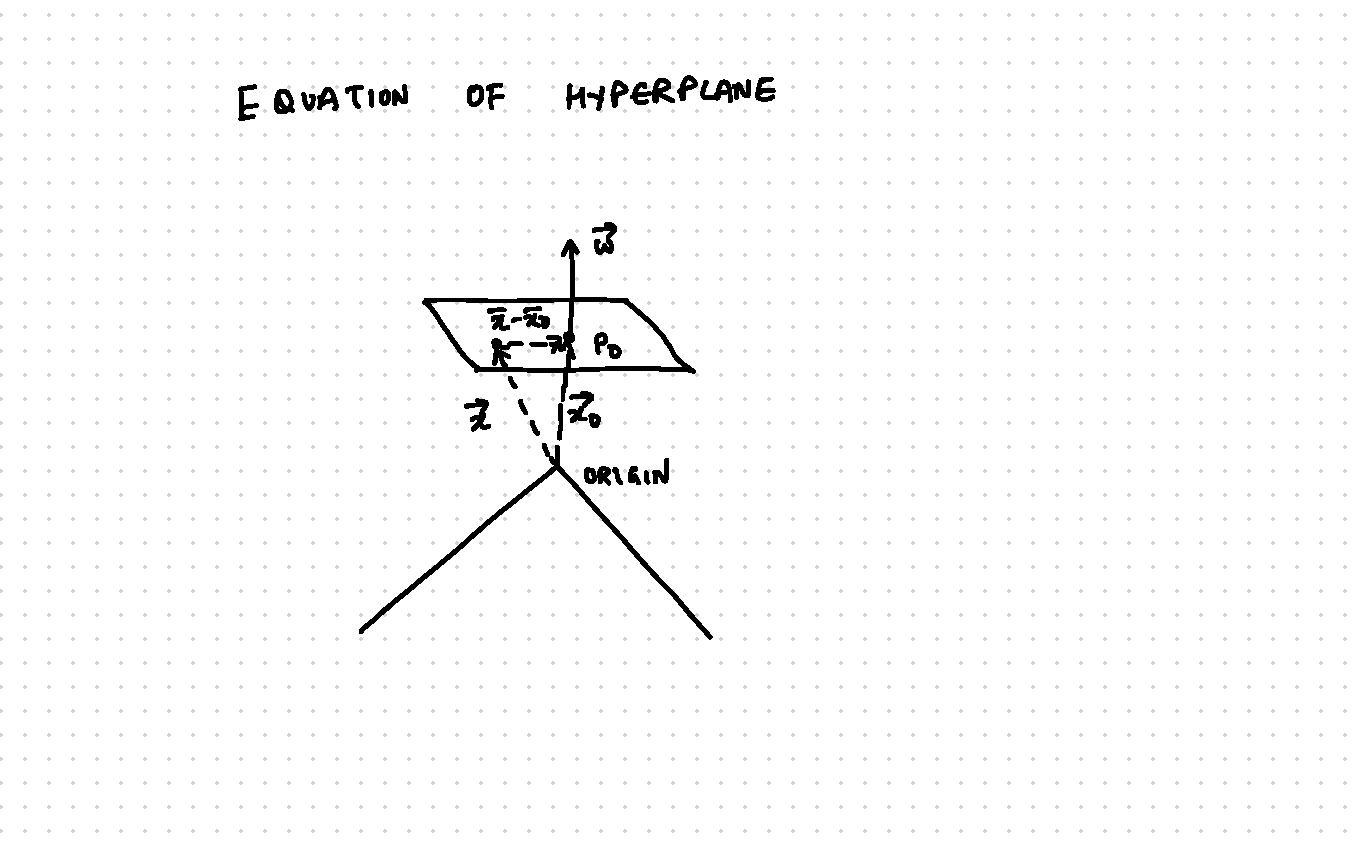
\includegraphics[scale=0.3]{./SVM/Svm-16.pdf}
\end{overprint}
\end{figure}


\end{frame}

\begin{frame}{Equation of Hyperplane}
 \begin{itemize}
	\item Defined by the point $P_{0}$ and the $\perp$ to the plane at that point $\overrightarrow{\text{w}}$
\end{itemize}
       \begin{tabular}{cl}  
         \begin{tabular}{c}
         
         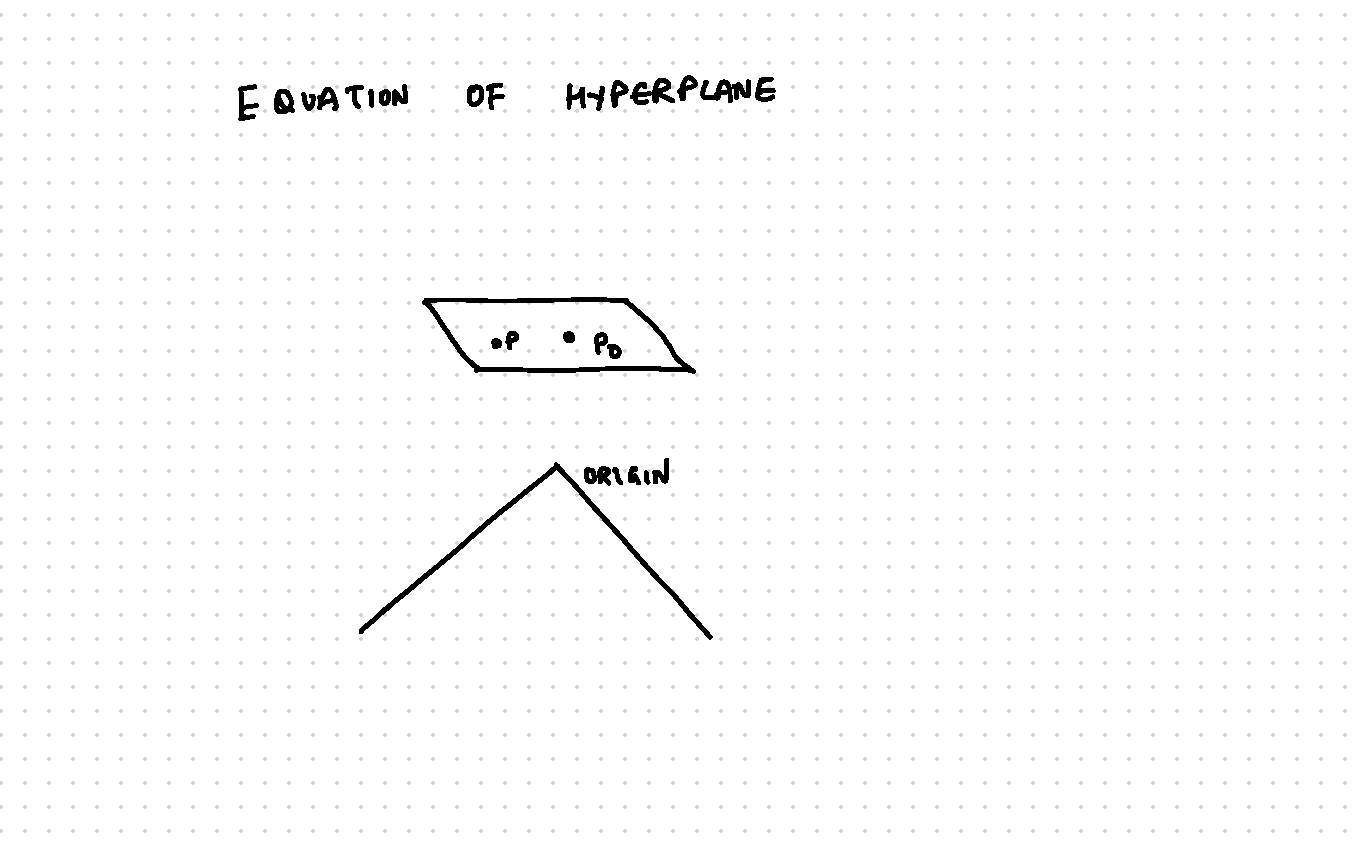
\includegraphics[scale = 0.25]{./SVM/Svm-13.pdf}
         
          \end{tabular}
          
          
        & \begin{tabular}{l}
             \parbox{0.5\linewidth}{
             \textbf{$P$, $P_{0}$ on plane} 

Now, 
 $w \perp \overrightarrow{\text{x}} - \overrightarrow{x_{0}}$\\
 $\Rightarrow w.(\overrightarrow{\text{x}} - \overrightarrow{x_{0}}) = 0$\\
 $\Rightarrow w.\overrightarrow{\text{x}} +  \overrightarrow{b} = 0$
 
    }
         \end{tabular}  \\
          
\end{tabular}
\end{frame}

\begin{frame}{An Example}

\begin{figure}
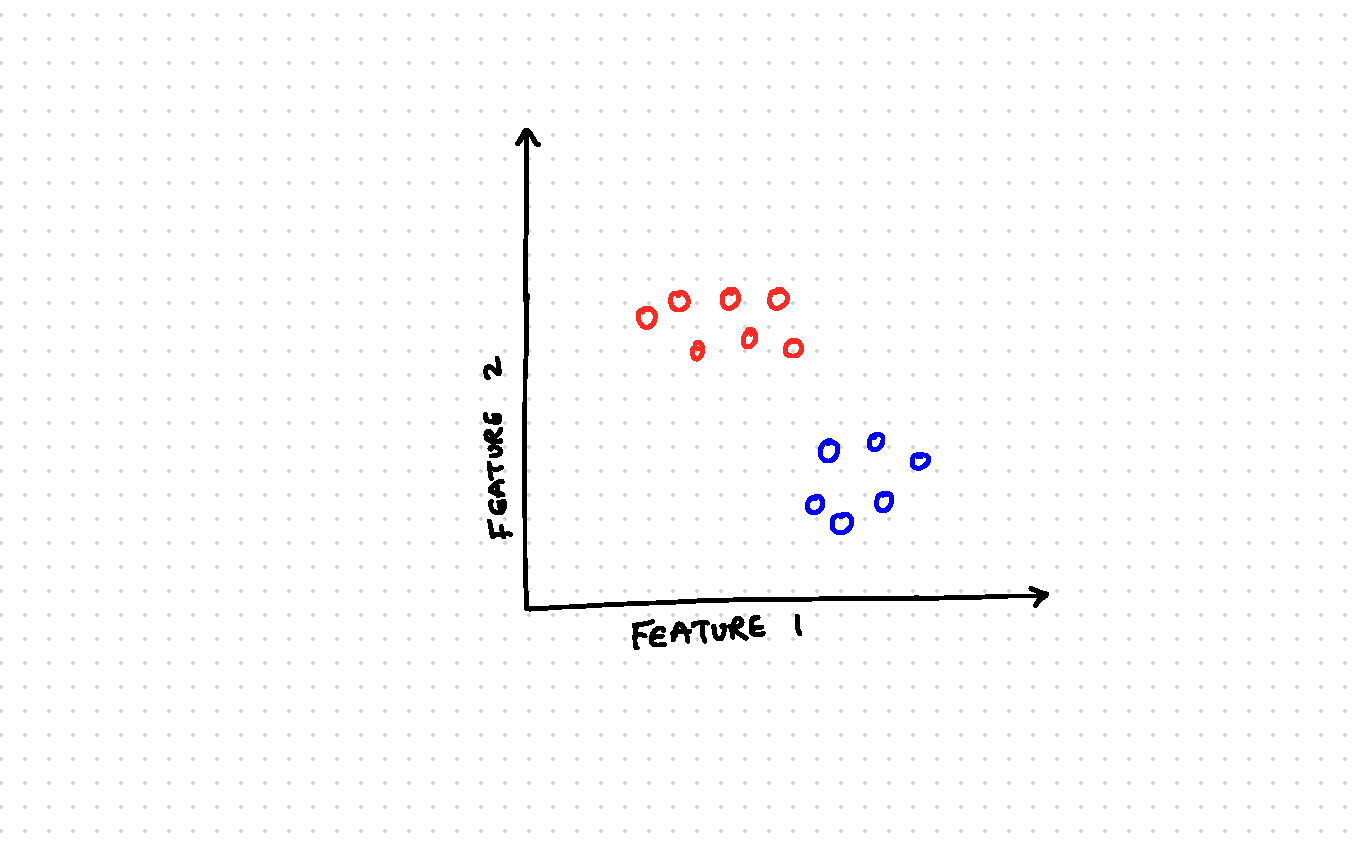
\includegraphics[scale=0.3]{SVM/Svm-1.pdf}
\end{figure}
$w = (2,1,4)$\\
$p_{0} = (0,2,3)$\\
$b = -w.x_{0} = (-2 \times 0 + 1 \times 2 + 4 \times 3) = -14$\\


\end{frame}

\begin{frame}{Distance between 2 parallel hyperplanes}

\begin{tabular}{cl}  
         \begin{tabular}{l}
         
         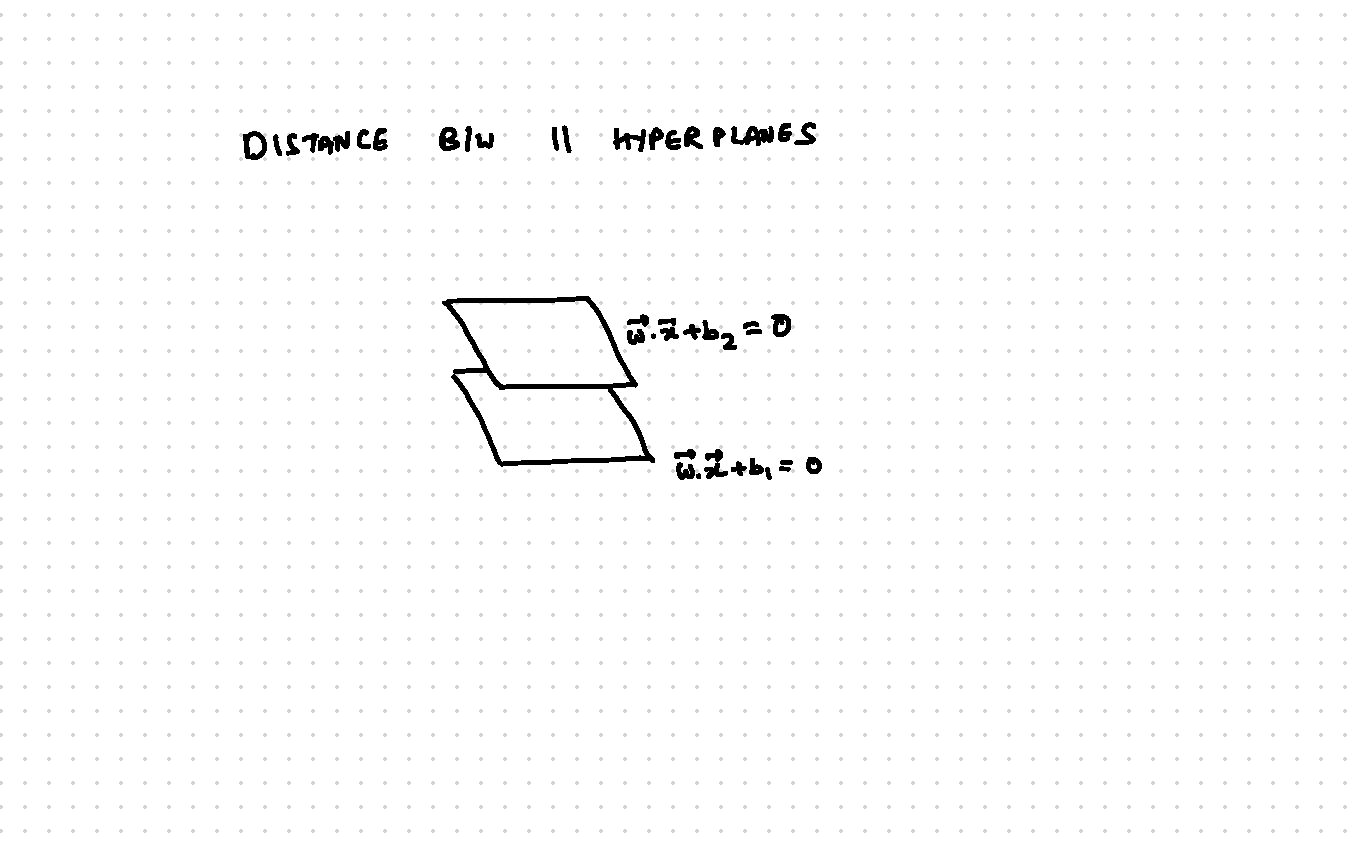
\includegraphics[height = 4cm, width = 5cm]{./SVM/Svm-17.pdf}
         
          \end{tabular}
          
          
        & \begin{tabular}{c}
             \parbox{0.5\linewidth}{
             \textbf{$P$, $P_{0}$ on plane} 

Now, 
 $w \perp \overrightarrow{\text{x}} - \overrightarrow{x_{0}}$\\
 $\Rightarrow w.(\overrightarrow{\text{x}} - \overrightarrow{x_{0}}) = 0$\\
 $\Rightarrow w.\overrightarrow{\text{x}} +  \overrightarrow{b} = 0$
 
    }
         \end{tabular}  \\
          
\end{tabular}

\end{frame}

\begin{frame}{Formulation}

\begin{figure}
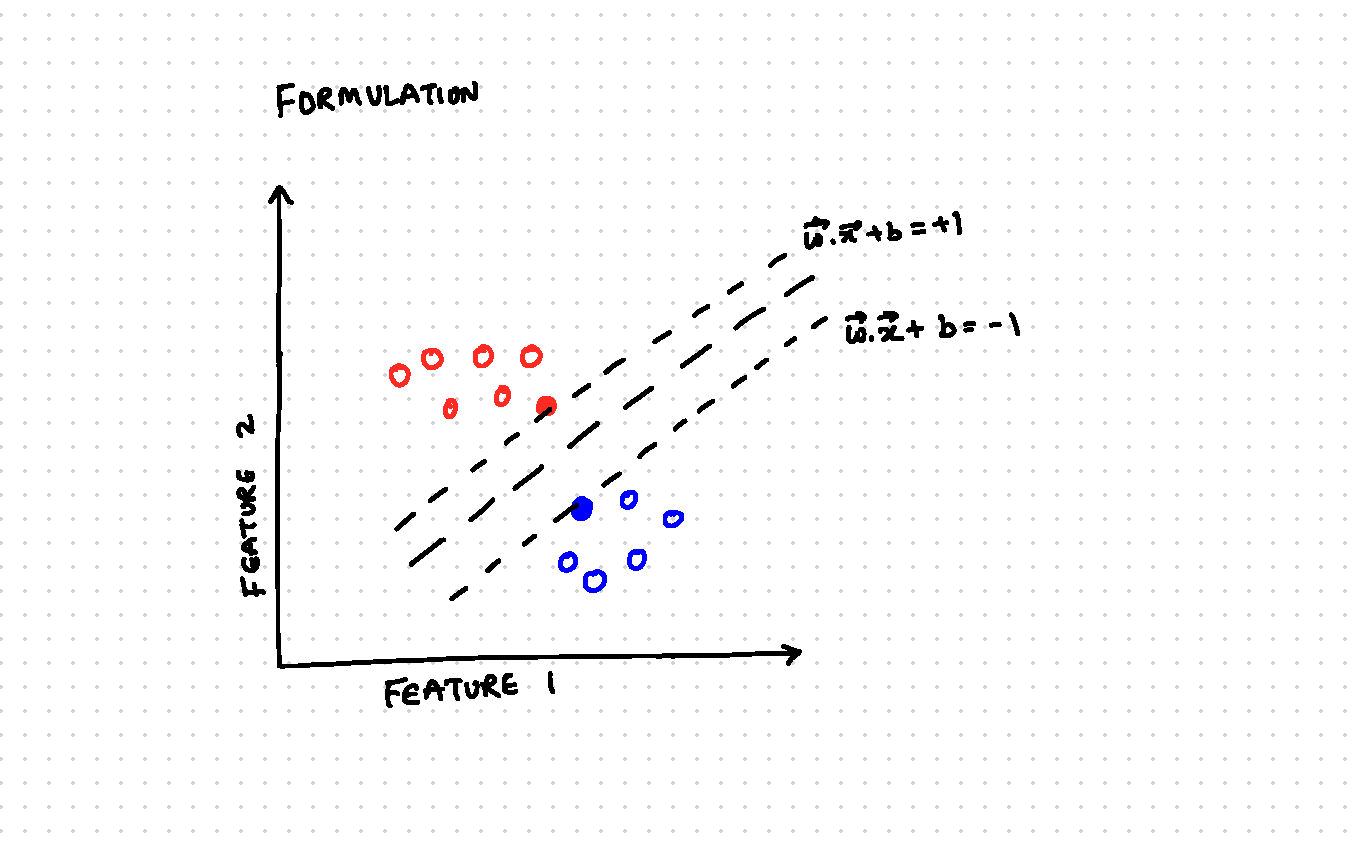
\includegraphics[scale=0.3]{SVM/Svm-20.pdf}
\end{figure}

\begin{itemize}
\item Margin $ = \frac{(b+1)-(b-1)}{||w||} = \frac{2}{||w||}$\
\item Goal is to Maximize margin $\Rightarrow$ minimize $||w||$

\end{itemize}

\end{frame}

\begin{frame}{Primal Formulation}
	\begin{tcolorbox}{Objective}
	\begin{align*}
	\text{Minimize } & \frac{1}{2}||w||^{2} \\
	\text{s.t. } & y_{i}(w.x_{i} + b) \geq 0 \hspace{2mm}\forall i
	\end{align*}
\end{tcolorbox}
\pause 
Q) What is $||w||$?
\pause
\begin{multicols}{2}
\begin{equation*}
	 w = \begin{bmatrix}
	 w_{1} \\
     w_{2} \\
     ...  \\
     w_{n} \\
	\end{bmatrix}
\end{equation*}\break
\begin{align*}
	 ||w|| &= \sqrt{w^{T}w}\\
	 &= \sqrt{\begin{bmatrix}
	 w_{1}, w_{2}, ... w_{n}
	 \end{bmatrix}
	 \begin{bmatrix}
	  w_{1} \\
	  w_{2} \\
     ...  \\
     w_{n} \\
	 \end{bmatrix}}
\end{align*}

\end{multicols}

\end{frame}

\begin{frame}{Simple Exercise}
\begin{multicols}{2}

\begin{figure}
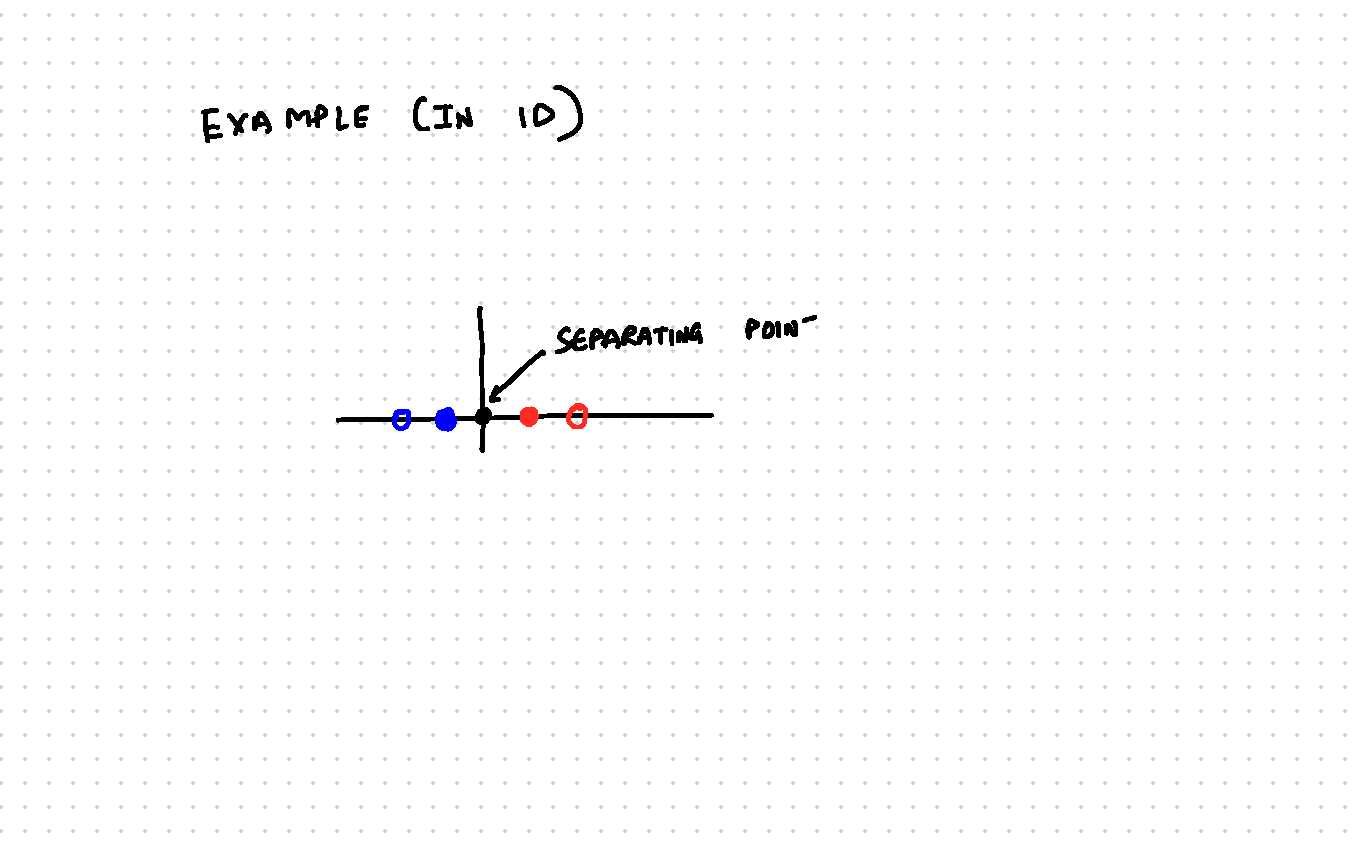
\includegraphics[scale = 0.25]{SVM/Svm-21.pdf}
\end{figure} \break
\vspace{10cm}
\begin{equation*}
\begin{bmatrix}
x_{1} && y \\
1 && 1\\
2 && 1\\
-1 && -1\\
-2 && -1\\
\end{bmatrix}
\end{equation*}

\end{multicols}
Separating Hyperplane: $w_{1}x_{1} + b = 0$

\end{frame}

\begin{frame}{Simple Exercise}
\begin{tcolorbox}

\begin{equation*}
y_{i}(w_{i}x_{i} + b) \geq 1
\end{equation*}
\end{tcolorbox}
\begin{multicols}{2}
\begin{equation*}
\begin{bmatrix}
x_{1} && y \\
1 && 1\\
2 && 1\\
-1 && -1\\
-2 && -1\\
\end{bmatrix}
\end{equation*}\break

\begin{align*}
&\Rightarrow y_{i}(w_{i}x_{i} + b) \geq 1\\
&\Rightarrow 1(w_{1} + b) \geq 1\\
&\Rightarrow 1(2w_{1} + b)\geq 1\\
&\Rightarrow -1(-w_{1}+b) \geq 1\\
&\Rightarrow -1(-2w_{1}+b) \geq 1\\
\end{align*}


\end{multicols}
\end{frame}

\begin{frame}{Simple Exercise}
\begin{multicols}{2}
\begin{figure}
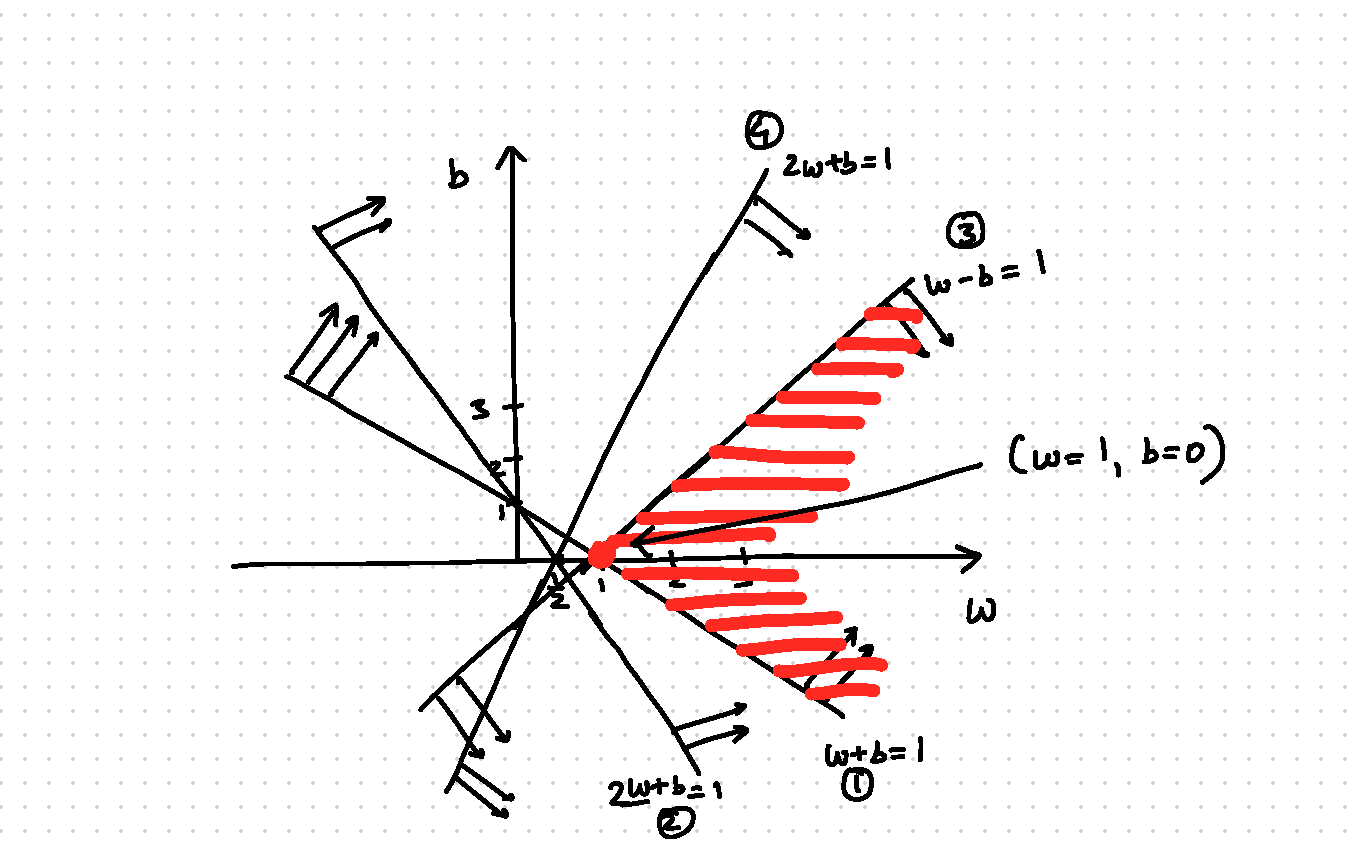
\includegraphics[scale=0.3]{SVM/Svm-27.pdf}
\end{figure}


\begin{align*}
&\Rightarrow 1(w_{1} + b) \geq 1\\
&\Rightarrow 1(2w_{1} + b)\geq 1\\
&\Rightarrow -1(-w_{1}+b) \geq 1\\
&\Rightarrow -1(-2w_{1}+b) \geq 1\\
\end{align*}

\end{multicols}

\begin{align*}
w_{min} = 1, b&= 0\\
w.x + b &= 0\\
x &=0 \\
\end{align*}

\end{frame}

\begin{frame}{Simple Exercise}
Minimum values satisfying constraints  $\Rightarrow$
$w_{1}$ = 1 and $b = 0$\\
$\therefore$ Max margin classifier $ \Rightarrow x = 0$

\end{frame}

\begin{frame}{Primal Formulation is a Quadratic Program}
\begin{align*}
\text{Generally;}&\\
&\Rightarrow \text{Minimize Quadratic(x)}\\
&\Rightarrow \text{such that, Linear(x)}
\end{align*}
\begin{multicols}{2}
\begin{tcolorbox}
Question
\begin{align*}
&{x} = (x_{1}, x_{2})\\
&\text{minimize} \hspace{3mm} \frac{1}{2}||x||^{2}\\
&\colon x_{1} + x_{2} - 1 \geq 0
\end{align*}
\end{tcolorbox}
\begin{figure}
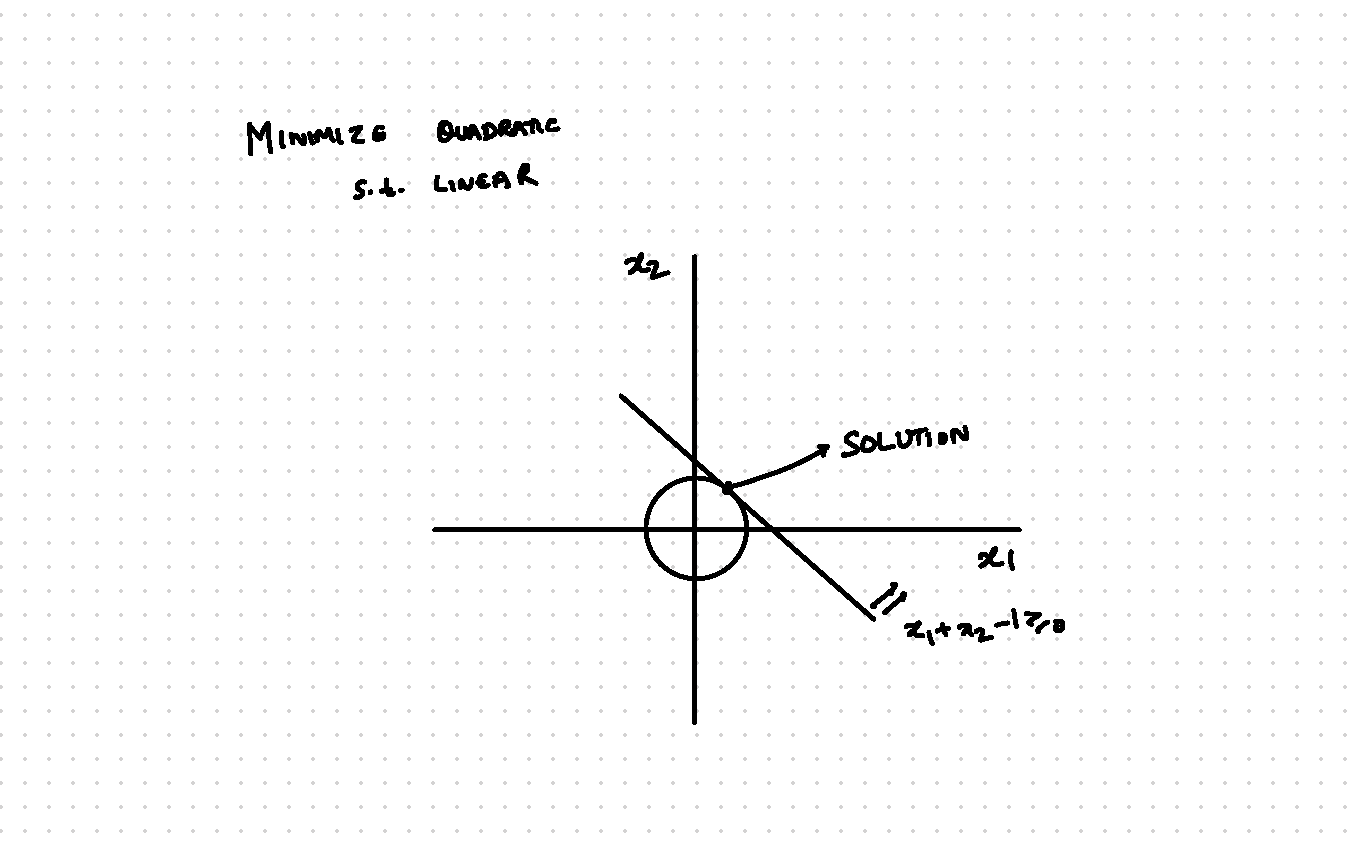
\includegraphics[scale=0.3]{SVM/Svm-28.pdf}
\end{figure}
\end{multicols}
\end{frame}

\begin{frame}{Converting to Dual Problem}
Primal $\Rightarrow$ Dual Conversion\\
\begin{align*}
	\text{Minimize } & \frac{1}{2}||\bar{w}||^{2} \\
	\text{s.t. } & y_{i}(\bar{w}.x_{i} + b) \geq 0 \hspace{2mm}\forall i
	\end{align*}
\begin{align*}
&L(\bar{w},b,\alpha_{1},\alpha_{2},...\alpha_{n}) = \frac{1}{2}
\sum_{i = 1}^{d} w_{i}^{2} - \sum_{i=1}^{N} \alpha_{i}(y_{i}(\bar{w}.\bar{x_{i}} + b) - 1) \hspace{2mm} \forall \hspace{2mm}\alpha_{i} \geq 0\\
&\frac{\partial L}{\partial b} = 0 \Rightarrow \sum_{i=1}^{n}\alpha_{i}y_{i} = 0\\
\end{align*}
\end{frame}

\begin{frame}{Converting to Dual Problem}
\begin{align*}
\frac{\partial L}{\partial w} = 0 \Rightarrow & \bar{w} - \sum_{i=1}^{n}\alpha_{i}y_{i}\bar{x_{i}} = 0\\
& \bar{w} = \sum_{i=1}^{N}\alpha_{i}y_{i}\bar{x_{i}}
\end{align*}
\begin{align*}
&L(\bar{w},b,\alpha_{1},\alpha_{2},...\alpha_{n}) = \frac{1}{2}
\sum_{i = 1}^{d} w_{i}^{2} - \sum_{i=1}^{N} \alpha_{i}(y_{i}(\bar{w}.\bar{x_i} + b) -1\\
&= \frac{1}{2}||\bar{w}||^{2}-\sum_{i=1}^{N} \alpha_{i} y_{i} \vec{w}_{.} \bar{x_{i}}-\sum_{i=1}^{N} \alpha_{i} y_{i} b+\sum_{i=1}^{N} \alpha_{i}\\
&= \sum_{=1}^{N} \alpha_{i}+\frac{\left(\sum_{i} \alpha_{i} y_{i} \bar{x}_{i}\right)\left(\sum_{j} \alpha_{j} y_{j} \bar{x}_{j}\right)}{2}-\sum_{i} \alpha_{i} y_{i}\left(\sum_{j} \alpha_{j} y_{j} \bar{x}_{j}\right) \bar{x_{i}}
\end{align*}
\end{frame}

\begin{frame}{Converting to Dual Problem}
\begin{align*}
&L(\alpha)=\sum_{i=1}^{N} \alpha_{i}-\frac{1}{2} \sum_{i=1}^{N} \sum_{j=1}^{N} \alpha_{i} \alpha_{j} y_{i} y_{j} \bar{x_{i}} \cdot \bar{x_{j}}\\
\end{align*}
\begin{tcolorbox}
\begin{align*}
&\begin{array}{ll}
{\text { Minimize }\|\bar{w}\|^{2} \Rightarrow}&{\text{Maximize } L(\alpha)} \\
{  s.t  } & {  s.t  } \\
{y_{i}\left(\bar{w}, x_{i}+b\right) \geqslant 1} & {\sum_{i=1}^{N} \alpha_{i} y_{i}=0 \hspace{2mm}\forall \hspace{2mm} \alpha_{i}  \geq 0}
\end{array}
\end{align*}
\end{tcolorbox}
\end{frame}

\begin{frame}{Question}
\textbf{Question}:\\
\vspace{2mm}
$\alpha_{i}\left(y_{i}\left(\bar{w}, \bar{x}_{i}+b\right)-1\right)=0 \quad \forall i$\\
\vspace{2mm}
What is $\alpha_{i}$ for support vector points?\\
\vspace{4mm}
\textbf{Answer:}
For support vectors,\\
\hspace{1in}$\bar{w}.\bar{x_{i}} + b  = -1$ (+ve class)\\
\hspace{1in}$\bar{w}.\bar{x_{i}} + b  = +1$ (+ve class)\\
\vspace{2mm}
$\left.y_{i}\left(\bar{w} \cdot \bar{x}_{i}+b\right)-1\right)=0 \quad \text {for } i=\{\text{support vector points\}}$
$\therefore \alpha_{i} \text { where i } \in \text{\{support vector points\}} \neq 0$
\vspace{5mm}
$\text{For all non-support vector points }\alpha_{i} = 0$
\end{frame}

\begin{frame}{Revisiting the Simple Example}
\begin{multicols}{2}

\begin{figure}
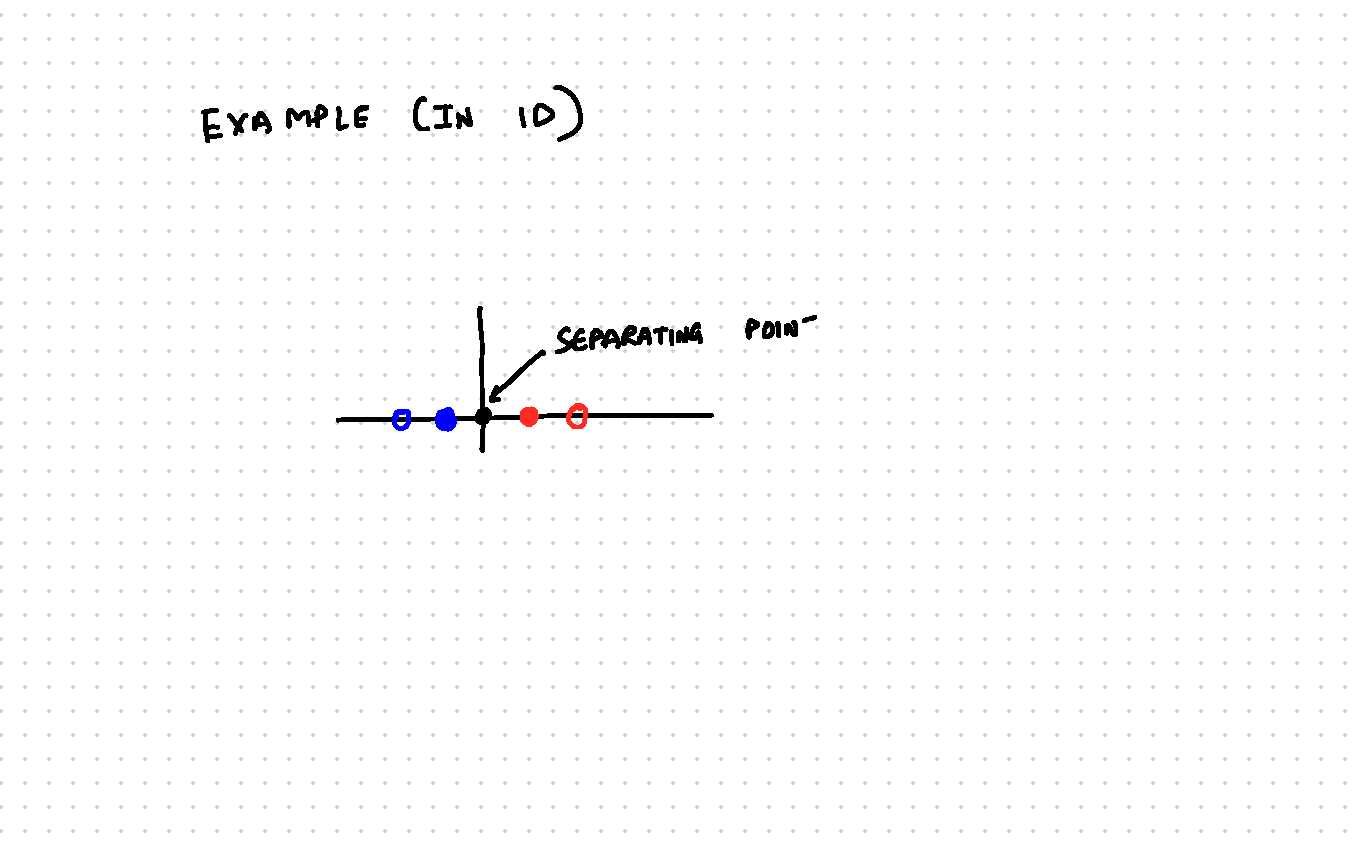
\includegraphics[scale = 0.25]{SVM/Svm-21.pdf}
\end{figure}

\begin{equation*}
\begin{bmatrix}
x_{1} && y \\
1 && 1\\
2 && 1\\
-1 && -1\\
-2 && -1\\
\end{bmatrix}
\end{equation*}
\end{multicols}
\begin{align*}
L(\alpha) &= \sum_{i=1}^{4} \alpha_{i} - \frac{1}{2}\sum_{i=1}^{4}\sum_{j=1}^{4}\alpha_{i}\alpha_{j}y_{i}y_{j}\bar{x_i}\bar{x_j} \hspace{1cm}\alpha_{i} \geq 0 \\
&\sum \alpha_{i}y_{i} = 0 \hspace{1.5cm}
\alpha_{i}(y_{i}(\bar{w}.\bar{x_i} + b - 1) = 0
\end{align*}

\end{frame}

\begin{frame}{Revisiting the Simple Example}
\begin{align*}
\begin{aligned}
\left.L(\alpha_{1},\alpha_{2},\alpha_{3},\alpha_{4}\right)=& \alpha_{1}+\alpha_{2}+\alpha_{3}+\alpha_{4} \\
&-\frac{1}{2}\left\{\alpha_{1} \alpha_{1}\times(1*1) \times(1 * 1)\right.\\
&\hspace{1cm} + \\
& \alpha_{1} \alpha_{2} \times(1*1) \times(1*2) \\
&\hspace{1cm}+\\
& \alpha_{1} \alpha_{3} \times(1*-1)\times(1*1)\\
& \hspace{1cm} ... \\
& \alpha_4\alpha_4 \times(-1*-1)\times(-2*-2)
\}
\end{aligned}
\end{align*}
How to Solve? $\Rightarrow$ Use the QP Solver!!
\end{frame}

\begin{frame}{Revisiting the Simple Example}
For the trivial example, \\
\hspace{2cm} By symmetry, $\alpha_{2} = \alpha_{4} = 0 $\text{ (say) }\\
\hspace{2cm} \& $\alpha_1 = \alpha_3  = 0$ \\
\hspace{2cm} \& $\sum y_i\alpha_i = 0$
\begin{align*}
\begin{aligned}
\left.L(\alpha_{1},\alpha_{2},\alpha_{3},\alpha_{4}\right)=& \alpha_{1}+\alpha_{2}+\alpha_{3}+\alpha_{4} \\
&-\frac{1}{2}\left\{\alpha_{2} \alpha_{4}(1)(-1)(2)(-2) \right. \\
&\hspace{1cm} +\\
& \alpha_{4} \alpha_{2}(-1)(1)(-2)(2) \\
\}\\
\end{aligned}
\end{align*}
\hspace{2cm} $\underset{\alpha}{Maximize} \hspace{3mm} 2\alpha - \frac{1}{2}(4\alpha^{2} + 4\alpha^{2})$
\end{frame}

\begin{frame}{Revisiting the Simple Example}
\begin{align*}
\begin{aligned}
\frac{\partial}{\partial \alpha}\left(2 \alpha-4 \alpha^{2}\right)=0 & \Rightarrow 2-8 \alpha=0 \\
\Rightarrow \hspace{2mm}& \alpha=1 / 4 \\
\end{aligned}\\
\therefore \alpha_{1}=0 \hspace{2mm} \alpha_{2}=\frac{1}{4} ; \hspace{2mm} \alpha_{3}=0 \hspace{2mm} \alpha_{4}=\frac{1}{4}
\\
\vec{w}=\sum_{i=1}^{N} \alpha_{i} y_{i} \bar{x}_{i} =0 \times 1 \times 1+\frac{1}{4} \times 1 \times 2 \\
+ 0 \times -1 \times -1 + \frac{1}{4}\times -1 \times -2 \\
 = 2/4 + 2/4 = 1
\end{align*}
\end{frame}

\begin{frame}{Revisiting the Simple Example}
\textbf{Finding b:}\\
For the support vectors we have, \\
$\alpha_{i}=0$\\
$\&$\\
$y_{i}(\vec{w} \cdot \overrightarrow{x_{i}}+b)-1=0$\\
or, $y_{i}$ $\left(\bar{w} \cdot \bar{x}_{1}+b\right)=1$\\
or, $y_{i}^{2}\left(\tilde{w} \cdot \tilde{x}_{i}+b\right)=y_{i}$\\
or, $\quad \bar{w}, \bar{x}_{i}+b=y_{i} \hspace{2mm}(\because y_{i}^{2} = 1)$\\
or, $b= y_i - w \cdot x_i$

\end{frame}

\begin{frame}{Obtaining the Solution}
\begin{align*}
\begin{aligned}
b &=\frac{1}{2}\{(1-(1)(1))+(-1-(1)(-1))\\
&=\frac{1}{2}\{0+0\}=0 \\
&=1 \\
& \therefore w = 1 \hspace{2mm}\& \hspace{2mm} b = 0
\end{aligned}
\end{align*}
\end{frame}

\begin{frame}{Making Predictions}
\textbf{Making Predictions} \\
\hspace{2cm} $\hat{y}(x_i) = \operatorname{SIGN}(w \cdot x_i + b)$\\
\begin{figure}
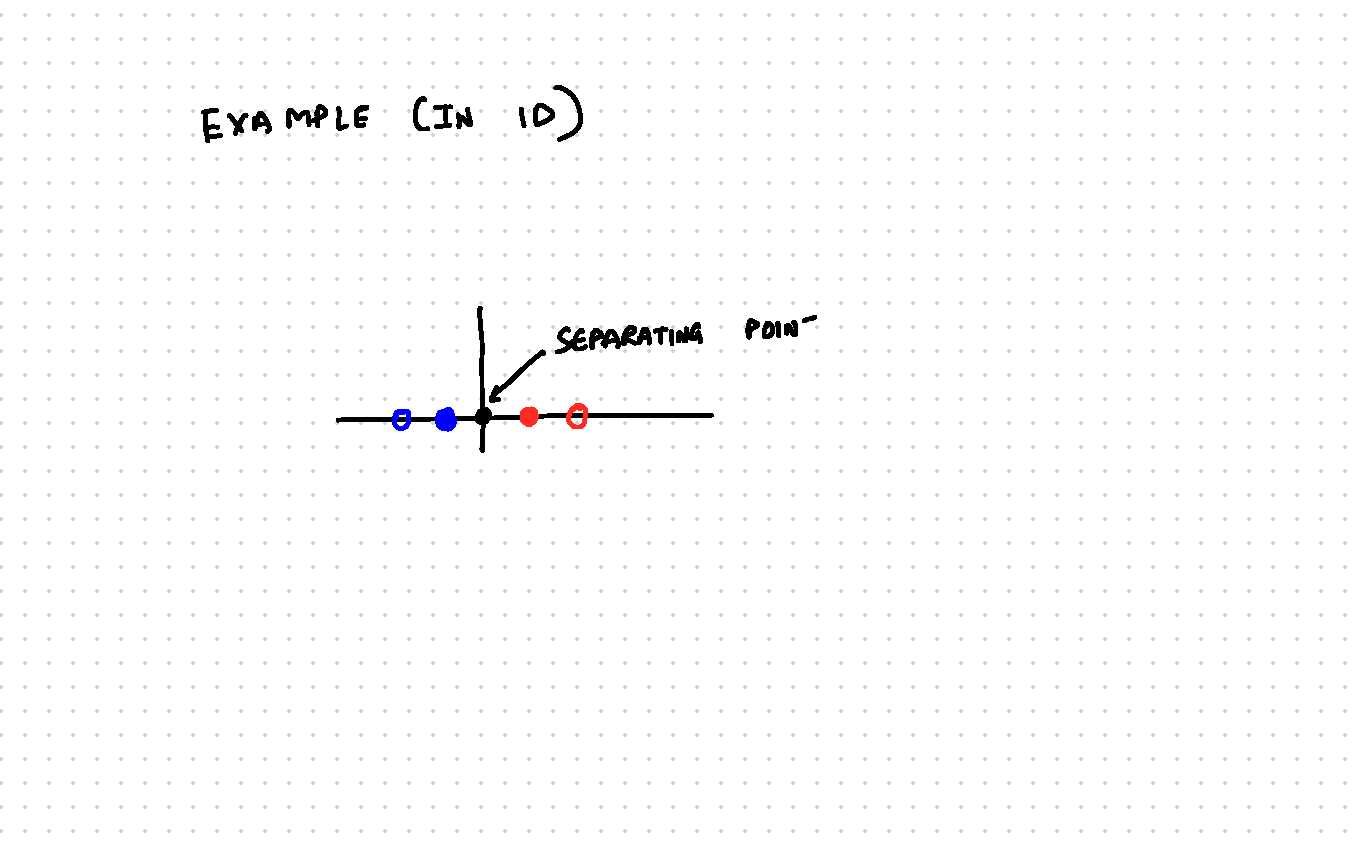
\includegraphics[scale = 0.3]{SVM/Svm-21.pdf}
\end{figure}
For $x_{test} = 3$; $\hat{y}(3) = \operatorname{SIGN}(1 \times 3 + 0)$ = +ve class
\end{frame}

\begin{frame}{Making Predictions}\
\begin{align*}
\begin{array}{l}
{\text {Alternatively, }} \\
{\qquad \begin{aligned}
\hat{y}\left(x_{TEST}\right) &=\operatorname{SIGN}\left(\bar{w} \cdot \bar{x}_{TEST}+b\right) \\
&=\operatorname{SIGN} \left(\sum_{i=1}^{N_{S}} \alpha_{j} y_{j} x_{j} \cdot x_{test}+b\right)
\end{aligned}}
\end{array}
\end{align*}
\begin{align*}
\begin{aligned}
&\text{In our example,} \\
&\alpha_{1}=0 ; \alpha_{2}=1 / 4 ; \quad \alpha_{3}=0 ; \alpha_{4}=1 / 4\\
&\hat{y}(3) =\operatorname{SIGN}\left(\frac{1}{4} \times 1 \times (2 \times 3)+0+\frac{1}{4} \times (-1) \times (-2 \times 3)+0\right)\\
&=\operatorname{SIGN} \left(\frac{12}{4}\right)=\operatorname{SIGN}(3)=+1
\end{aligned}
\end{align*}

\end{frame}
\end{document}